\documentclass[12pt, oneside]{article}
\usepackage[letterpaper, margin=1in, headsep=0.5in]{geometry}
\usepackage[english]{babel}
\usepackage[utf8]{inputenc}
\usepackage{amsmath}
\usepackage{amsfonts}
\usepackage{amssymb}
\usepackage{tikz}
\usetikzlibrary{quotes, angles}
\usepackage{graphicx}
%\usepackage{pgfplots}
%\pgfplotsset{width=10cm,compat=1.9}
%\usepgfplotslibrary{statistics}
%\usepackage{pgfplotstable}
%\usepackage{tkz-fct}
%\usepackage{venndiagram}
\usepackage{multicol}

\usepackage{fancyhdr}
\pagestyle{fancy}
\fancyhf{}
\rhead{\thepage \\Name: \hspace{1.5in}.\\}
\lhead{BECA / Dr. Huson / 10.3 Geometry\\* 22 May 2019}

\renewcommand{\headrulewidth}{0pt}

\begin{document}
  \begin{enumerate}
    \subsubsection*{Do Now: Graphing practice}

        \item Graph the line $y=\frac{3}{2} x -4$ after filling in the values in the blanks.\\[0.85cm]
              $y$-intercept $= \rule{2cm}{0.15mm}$ \\[0.5cm]
              Slope $= \rule{2cm}{0.15mm}$\\

        \begin{center} %4 quadrant regents grid w T-Chart
        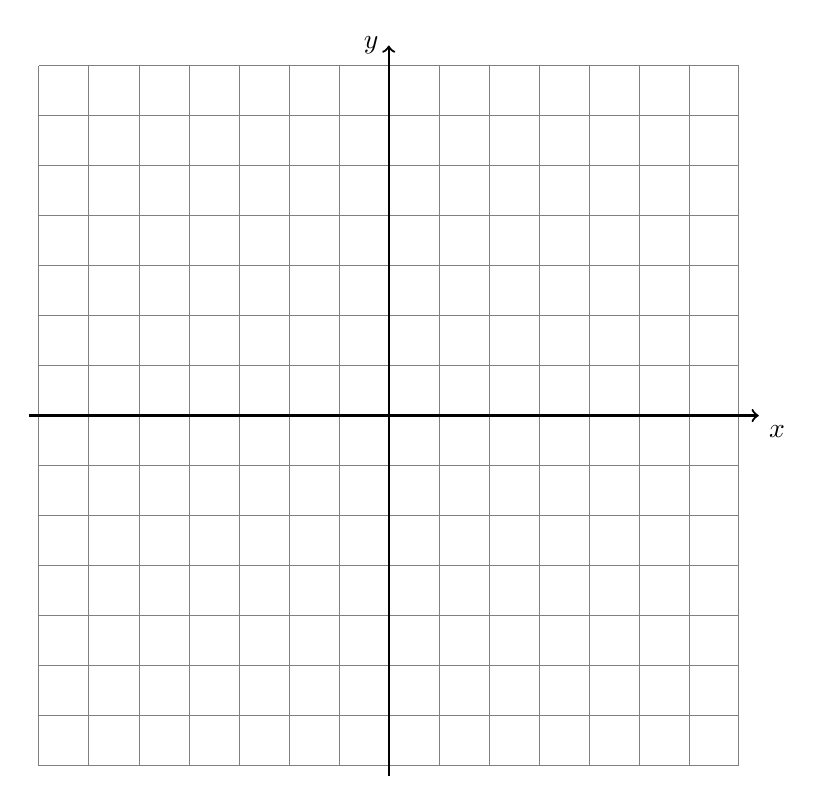
\begin{tikzpicture}[scale=.635]
          \draw [help lines] (-7,-7) grid (7,7);
          \draw [thick, ->] (-7.2,0) -- (7.4,0) node [below right] {$x$};
          \draw [thick, ->] (0,-7.2)--(0,7.4) node [left] {$y$};
        \end{tikzpicture}
        \end{center}

        In the following two problems, solve for the value of $x$.
        \begin{multicols}{2}
        \item   $x-4=3x-4$ \vspace{3cm}
        \item   $\frac{1}{3}(6-9x)=-1$ %\vspace{3cm}
        \end{multicols}

\newpage
\item Graph the two inequalities. Write an ``S" to mark the solution set.\\[0.5cm]

  \begin{multicols}{2}
    $y \geq \frac{1}{3} x -3$ \\
    $y < -x +5$
  \end{multicols}
  \begin{center} %4 quadrant regents grid w T-Chart
  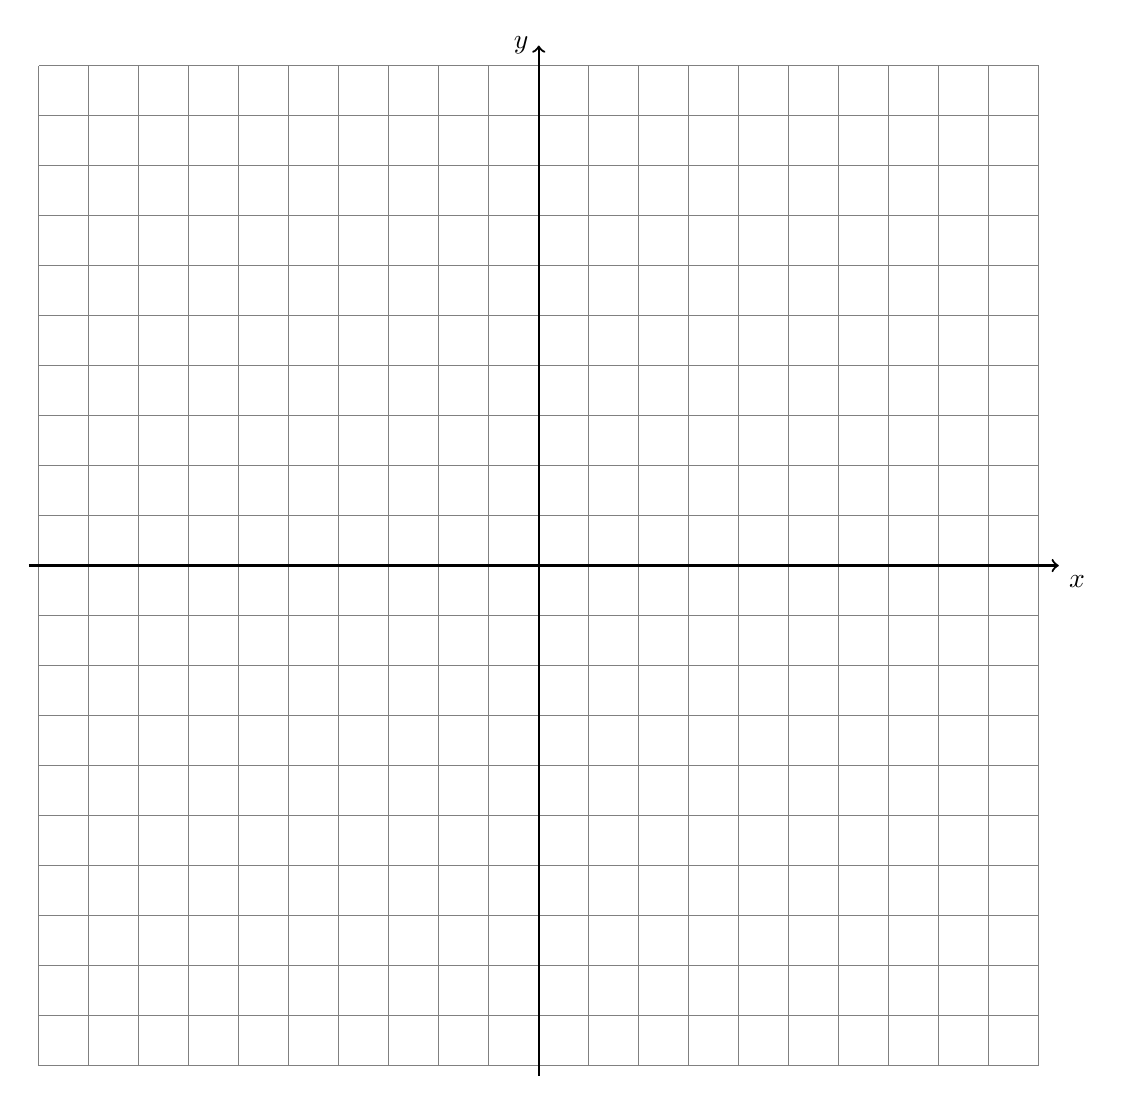
\begin{tikzpicture}[scale=.635]
    \draw [help lines] (-10,-10) grid (10,10);
    \draw [thick, ->] (-10.2,0) -- (10.4,0) node [below right] {$x$};
    \draw [thick, ->] (0,-10.2)--(0,10.4) node [left] {$y$};
  \end{tikzpicture}
  \end{center}

  Solve each equation for $y$.
  \begin{multicols}{2}
    \raggedcolumns
    \begin{enumerate}
      \item $2x+y=5$\\[0.5cm]
    \end{enumerate}
    \begin{enumerate}
      \item $3x-6y=12$ \\[0.5cm]
    \end{enumerate}
  \end{multicols}

  \newpage


\subsubsection*{Fitting linear models and interpreting correlation}
\item Dr. Huson is saving money each week in his piggy bank. The amount in his bank after a number of weeks is shown in the table.
  \renewcommand{\arraystretch}{1.6}
    \begin{center}
      \begin{tabular}{|l|r|r|r|r|}
      \hline
      Weeks & 3 & 5 & 6 & 10\\
      \hline
      Savings  & \$15.00 & 20.00 & 21.50 & 29.00 \\
      \hline
      \end{tabular}
    \end{center}

\begin{center} %4 quadrant regents grid w T-Chart
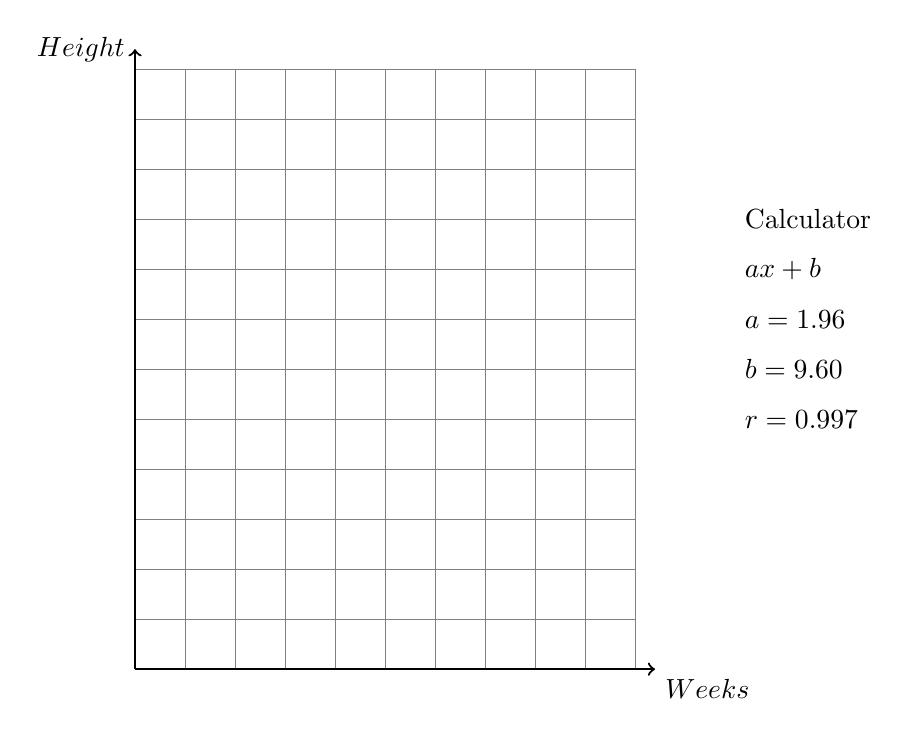
\begin{tikzpicture}[scale=.635]
  \draw [help lines] (0,0) grid (10,12);
  \draw [thick, ->] (0,0) -- (10.4,0) node [below right] {$Weeks$};
  \draw [thick, ->] (0,0)--(0,12.4) node [left] {$Height$};
  \node at (12,9)[right]{Calculator};
  \node at (12,8)[right]{$ax+b$};
  \node at (12,7)[right]{$a=1.96$};
  \node at (12,6)[right]{$b=9.60$};
  \node at (12,5)[right]{$r=0.997$};
\end{tikzpicture}
\end{center}
State, to the \emph{nearest tenth}, the linear regression equation that approximates the savings balance, $y$, after $x$ weeks.\\[2cm]
Explain what the $y$-intercept means in the context of the problem. \\[3cm]
Explain what the slope means in the context of the problem.
\newpage
\subsubsection*{Simplifying polynomials, standard form}

\item Simplify the expresion $2x + 3(x+5)+4$.\vspace{4cm}
\item Write the expression $3x+2x^2-6x^2+9x+5+3x$ as a polynomial in standard form. \vspace{7cm}

  \item Write the expression $5x+4x^2(2x+7)-6x^2-9x$ as a polynomial in standard form.

\newpage


\subsubsection*{Graphing quadratic functions}

\item Given the quadratic function $f(x)=x^2+1$, find the row differences.
  \renewcommand{\arraystretch}{1.6}
    \begin{center}
      \begin{tabular}{|c|r|}
      \hline
      $x$ & $f(x)$\\
      \hline
      -3 & 10 \\
      \hline
      -2 & 5 \\
      \hline
      -1 & 2 \\
      \hline
      0 & 1 \\
      \hline
      1 & 2 \\
      \hline
      2 & 5 \\
      \hline
      3 & 10 \\
      \hline
      \end{tabular}
    \end{center}
Graph the function as a line over the domain $-3 \leq x \leq 3$.

\begin{center} %4 quadrant regents grid w T-Chart
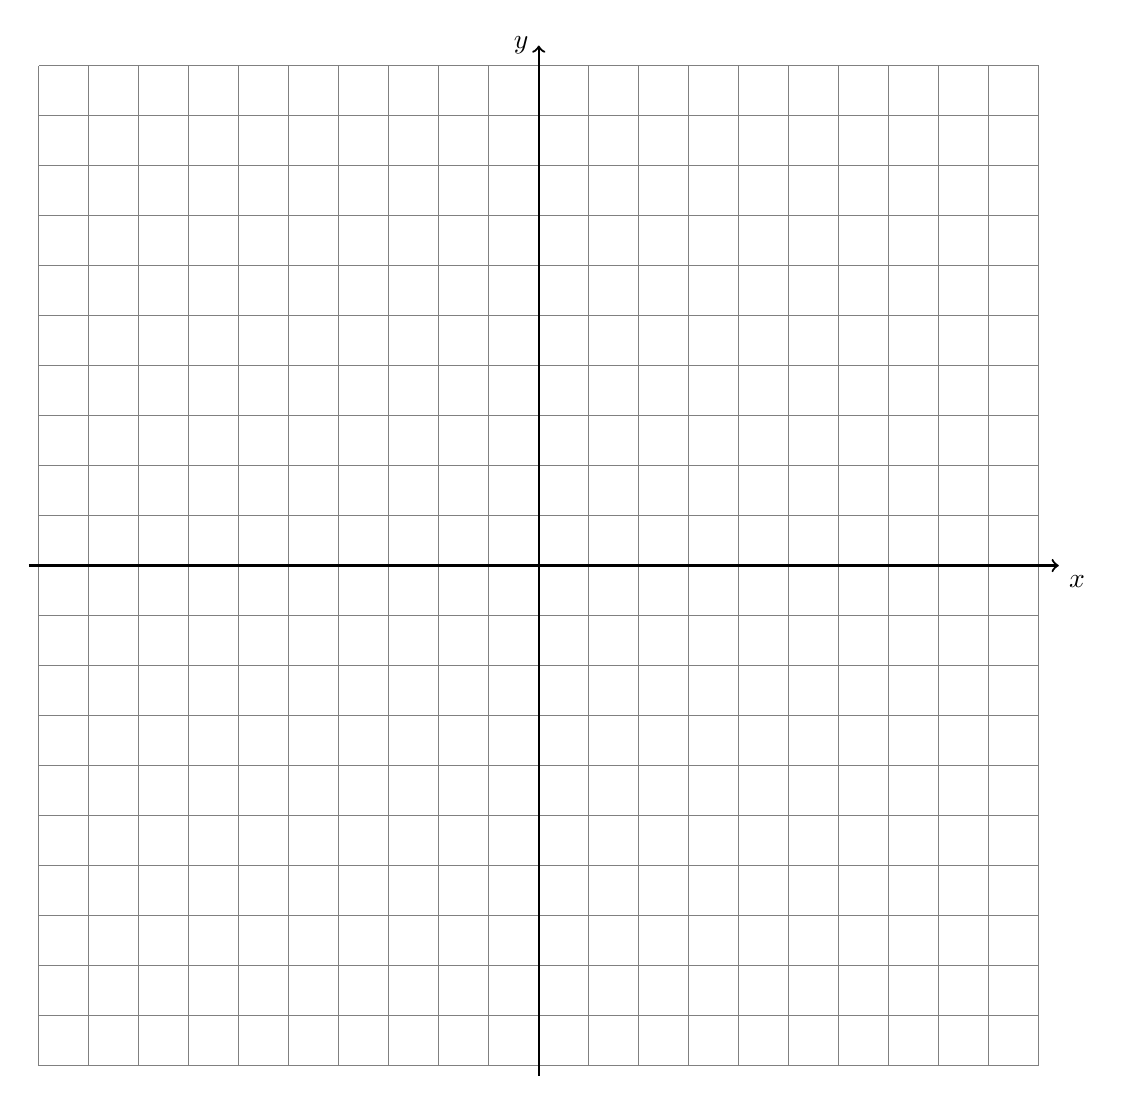
\begin{tikzpicture}[scale=.635]
  \draw [help lines] (-10,-10) grid (10,10);
  \draw [thick, ->] (-10.2,0) -- (10.4,0) node [below right] {$x$};
  \draw [thick, ->] (0,-10.2)--(0,10.4) node [left] {$y$};
\end{tikzpicture}
\end{center}

\newpage
\subsection*{Rate of change}

\item Find the slope of the function from the ratio of the line differences.

  \begin{multicols}{2}
  \begin{enumerate}
    \item
      \begin{tabular}{|c|r|}
      \hline
      $x$ & $f(x)$\\
      \hline
      -2 & -1 \\
      \hline
      -1 & 1 \\
      \hline
      0 & 3 \\
      \hline
      1 & 5 \\
      \hline
      2 & 7 \\
      \hline
      \end{tabular}\\[0.85cm]

      Change in $y$ $= \rule{2cm}{0.15mm}$ \\[0.5cm]
      Change in $x$ $= \rule{2cm}{0.15mm}$ \\[0.5cm]
      Slope $= \rule{2cm}{0.15mm}$\\


    \item
      \begin{tabular}{|c|r|}
      \hline
      $x$ & $f(x)$\\
      \hline
      -4 & 7 \\
      \hline
      -2 & 4 \\
      \hline
      0 & 1 \\
      \hline
      2 & -2 \\
      \hline
      4 & -5 \\
      \hline
      \end{tabular}\\[0.85cm]

      Change in $y$ $= \rule{2cm}{0.15mm}$ \\[0.5cm]
      Change in $x$ $= \rule{2cm}{0.15mm}$ \\[0.5cm]
      Slope $= \rule{2cm}{0.15mm}$\\

    \end{enumerate}
    \end{multicols}

  \item Find the slope of the function. If the rate of change is not constant, write, ``Non-linear. The rate of change is not constant."

    \begin{multicols}{2}
    \begin{enumerate}
      \item
        \begin{tabular}{|c|r|}
          \hline
          $x$ & $f(x)$\\
          \hline
          -3 & 0 \\
          \hline
          -1 & 2 \\
          \hline
          0 & 3 \\
          \hline
          1 & 4 \\
          \hline
          3 & 6 \\
          \hline
        \end{tabular}\\[0.85cm]

        Slope $= \rule{2cm}{0.15mm}$\\


      \item
        \begin{tabular}{|c|r|}
          \hline
          $x$ & $f(x)$\\
          \hline
          -4 & -9 \\
          \hline
          -2 & -3 \\
          \hline
          0 & +1 \\
          \hline
          2 & -3 \\
          \hline
          4 & -9 \\
          \hline
        \end{tabular}\\[0.85cm]

        Slope $= \rule{2cm}{0.15mm}$\\

      \end{enumerate}
    \end{multicols}

\newpage


\item Fill in the T-chart, plot the points, and draw the line.

    \begin{center} %4 quadrant regents grid w T-Chart
    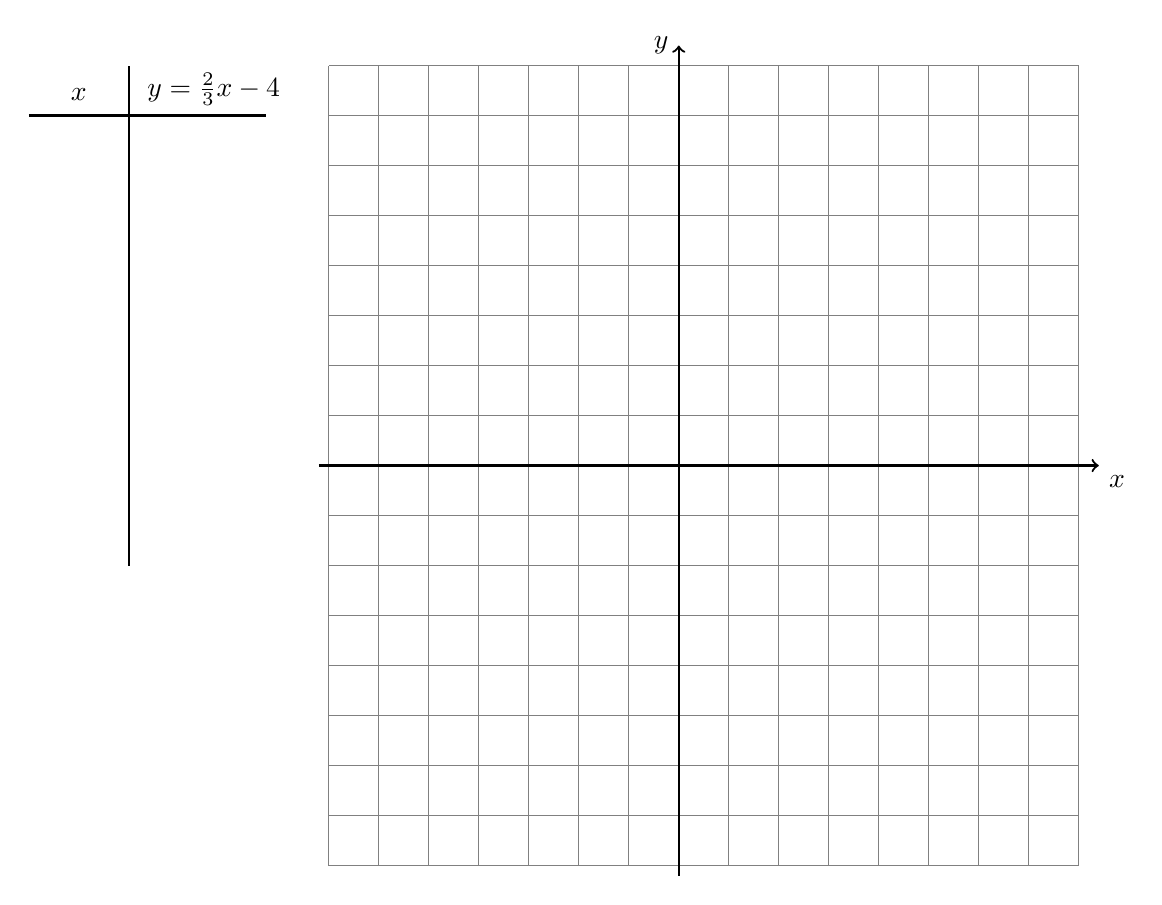
\begin{tikzpicture}[scale=.635]
      \draw [thick, -] (-11, -2)--(-11,8);
      \draw [thick, -] (-13,7)--(-8.25,7);
      \node at (-12,7.1) [above] {$x$};
      \node at (-9.3,7) [above] {$y=\frac{2}{3}x-4$};
      \draw [help lines] (-7,-8) grid (8,8);
      \draw [thick, ->] (-7.2,0) -- (8.4,0) node [below right] {$x$};
      \draw [thick, ->] (0,-8.2)--(0,8.4) node [left] {$y$};
    \end{tikzpicture}
    \end{center}
Write down the slope and $y$-intercept of the line.\\[0.5cm]
$m=$\\[0.5cm]
$b=$\\[0.5cm]
Circle the row for the $y$-intercept.


\end{enumerate}
\end{document}
